\documentclass[../thesis/thesis.tex]{subfiles}
\begin{document}
\chapter{Architecture}

Since the advent of a standardised \iot protocol stack discussed in \Fref{sec:litreview:architecture}, the decision making process for protocol architecture has been simplified immensely. As a key part of an effective Thing is interoperability, it is clear that adopting the standardised protocol stack is the way forward. As such, the proposed protocol architecture described in \Fref{tab:litreview:protostack} will form the stack used by the ``WPAN'' network shown in \Fref{fig:litreview:devices}.

Moving from a protocol perspective to a device perspective, when one considers the energy efficiency and cost constrains of this project, it is clear that a system in which low-powered and cheap embedded systems, such as Arduinos, are the best choice for each of the sensing nodes. This recognises the fact that these nodes have computationally complex tasks, and are merely responsible for the transmission of the collected data.

As a natural consequence of choosing simple sensing nodes, a more powerful processing node must be added to the system to collect the unprocessed data produced by the sensing nodes and interpret it into the high-level occupancy answers this project wishes to provide. As such a node does not need to be in a particular location (provided it is in range of the sensor WPAN), it does not need to be as considerate of low power requirements. A primary hardware candidate for this node is the Raspberry Pi. Advantages include it still being quite low powered, built-in support for WPAN networking expansion cards, and traditional built-in LAN networking. These characteristics also allow it to act as the ``smart gateway'' between the sensors and the broader \iot.

% TODO: Normalize accuracy stats


\section{Ideal System Architecture}
\label{sec:litreview:architecture}
Beyond specific sensor design and occupancy detection algorithms, a core goal of this project is to create a system that is designed to operate as a useful Thing in a real-world \iot environment, as the key advantage of Things is the ``disruptive level of innovation''\cite{atzori2010internet} brought about by their ability to be combined in ways unforeseen (yet still enabled) by their creators. This architecture involves careful consideration of the embedded hardware that will drive the system, as well as the communications protocols utilised between the sensor and devices interested in the sensor's information.

\subsection{Protocols}
\label{subsec:litreview:architecture:protocols}
% From; https://openwsn.atlassian.net/wiki/pages/viewpage.action?pageId=29196353
\begin{table}
\centering
\begin{tabular}{|c|c|}
\hline
\multicolumn{2}{|c|}{\acs{rest}} \\ \hline
\textbf{Application} & \acs{coap} \\ \hline
\textbf{Transport} & UDP \\ \hline
\textbf{IP / Routing} & IETF \acs{roll} \\ \hline
\textbf{Adaptation} & IETF \acs{lowpan} \\ \hline
\textbf{Medium Access} & IEEE \lmed \\ \hline
\textbf{Physical} & IEEE \lphy \\ \hline
\end{tabular}
\caption{Proposed protocol stack}
\label{tab:litreview:protostack}
\end{table}

In an ideal smart-home environment, the sensor systems used will communicate with each other wirelessly. As the complete sensor system has low power requirements to enable battery operation, it is important to prioritise those protocols and architectures that minimise power usage while still enabling the necessary wireless communication. The system will also ideally exist in a system with other identical sensors (one for each room in a residence), thus it is important to prioritise those protocols which allow multiple identical sensor systems to coexist on the same network without conflict, and to be uniquely addressable and identifiable. In recent years, many developments have been made in the \iot arena, with standards emerging specifically designed for low-power embedded devices to communicate between themselves and bigger systems that address these and other unique needs, across the entire protocol stack. 

Palattella \etal \cite{palattella2013standardized} propose a protocol stack that aligns with the above requirements, with the key advantage being a wholly standardized implementation of the stack exists. This implementation is based on TCP/IP, uses the latest IEEE and IETF \iot standards, and is free from proprietary protocol restrictions (unlike ZigBee 1.0 devices, for instance). \Fref{tab:litreview:protostack} shows the full stack proposed. The key components of this proposal are the introduction of \acs{coap} at the application layer, \acs{roll} at the IP / Routing layer and \acs{lowpan} at the Adaptation layer.

Above the application layer, Guinard \etal \cite{guinard2012search} propose the use of \rest over \ws as a method of exchanging information between sensor systems. Their data suggests that \rest is easier to use than \ws, and the key advantage of a \ws based approach is its ability to represent much more complex data and abstractions, which are unnecessary in this project's situation.

\coap \cite{kovatsch2013coap} is an application layer protocol designed to replace HTTP as a way of transmitting RESTful information between clients. The chief advantage of \coap over HTTP is it compresses the broad-strokes of the HTTP feature set into a binary language that is much more suitable for transmission over low-bandwidth and low-power links, such as those discussed here.

\roll \cite{rfc6550} is a routing protocol designed for low power environments, allowing low power nodes to create and maintain a mesh network between themselves, allowing, among other things, the routing of packets to a ``root'' node and back again. \roll is particularly suited to the routing situation of our proposed architecture, as individual sensors do not need to communicate with one another, but rather report back to a larger node (further discussed in \Fref{subsec:litreview:architecture:devices}).

\lowpan \cite{shelby20116lowpan} is a compression and formatting specification to allow IPv6 packets to be sent over an \lwifi based network. Optimisations are found in the reduction of the size of \lowpan packets, IPv6 addresses as well as redesigning core Internet Protocol algorithms so that they can run with low power consumption on participating devices.

\subsection{Devices}
\label{subsec:litreview:architecture:devices}
\begin{figure}
\centering
\begin{tikzpicture}[node distance=1.7cm]
\node (interwebs) [cbox] {Internet};
\node (http) [dashbox, left=of interwebs] {\small HTTP};
\node (rpi) [box, below=of http] {Smart Gateway / Processor};
\node (coap) [dashbox, right=of rpi] {\small \acs{coap}};
\node (mesh) [cbox, right=of coap] {WPAN};
\node (embed1) [box, below left=of mesh] {Sensor};
\node (embed2) [box, below right=of mesh] {Sensor};

\draw [line] (interwebs) -- (http);
\draw [line] (http) -- (rpi);
\draw [line] (rpi) -- (coap);
\draw [line] (coap) -- (mesh);
\draw [line] (mesh) -- (embed1);
\draw [line] (mesh) -- (embed2);
\end{tikzpicture}
\caption{Proposed system architecture}
\label{fig:litreview:devices}
\end{figure}

In addition to the protocol stack used, how these nodes relate to each other is also an important consideration. Part of what will inform these decisions are the requisite processing power and internet connectivity required to successfully execute all elements of the sensing system. Kovatsch \cite{kovatsch2013coap} provides a constructive classification system to consider this, by describing three classes of resource constrained devices that would benefit from \coap, and each can provide different levels of security for an IP stack;

\begin{itemize}
 \item \emph{Class 0}: ``not capable of running an RFC-compliant IP stack in a secure manner. They require application-level gateways to connect to the Internet.''
 \item \emph{Class 1}: Able to connect to the internet with some ``integrated security mechanisms''. Are unable to employ full HTTP with TLS.
 \item \emph{Class 2}: Normal Internet nodes, able to use the full HTTP stack with TLS.
\end{itemize}

The devices that we propose the sensors will connect to are the likes of the Arduino, which can be classified as class 0 or possibly class 1 devices. Due to their insecurity and difficulty running a fully fledged IP stack, Guinard \etal \cite{guinard2011internet} propose the use of a ``Smart Gateway'' system to bridge the wider internet and these sensor systems. This gateway would be able to communicate with the sensor systems over \coap and \lwifi, as well as receive API requests via HTTP from a traditional TCP/IP network to forward on to these sensors.

The Thermosense paper \cite{beltran2013thermosense} proposes several different algorithms to process the raw sensing data into the occupancy estimates (further discussed in \Fref{sec:litreview:thermalsensors}), all of which are fairly computationally expensive. Because of this, it would be non-trivial to implement these algorithms on the embedded sensing devices themselves. This problem is already resolved in our proposed system, as the aforementioned ``Smart Gateway'' can easily also take on the task of processing the raw sensor data into estimates which it can relay to interested parties over its HTTP-based API. A visualisation of this proposed system is shown in \Fref{fig:litreview:devices}.

\section{Prototype System Architecture}
Due to limited time available, parts of the above ideal system architecture have been deemed outside of the scope of the project. To help achieve appreciable results in the time available, the use of wireless mesh networking and the support of a one-to-many ``smart gateway'' to sensor has not been explored. However, as discussed below, the prototype architecture selected as been designed such that a clear path to the idea system architecture is available.

\subsection{Hardware}
 
\begin{figure}
\centering
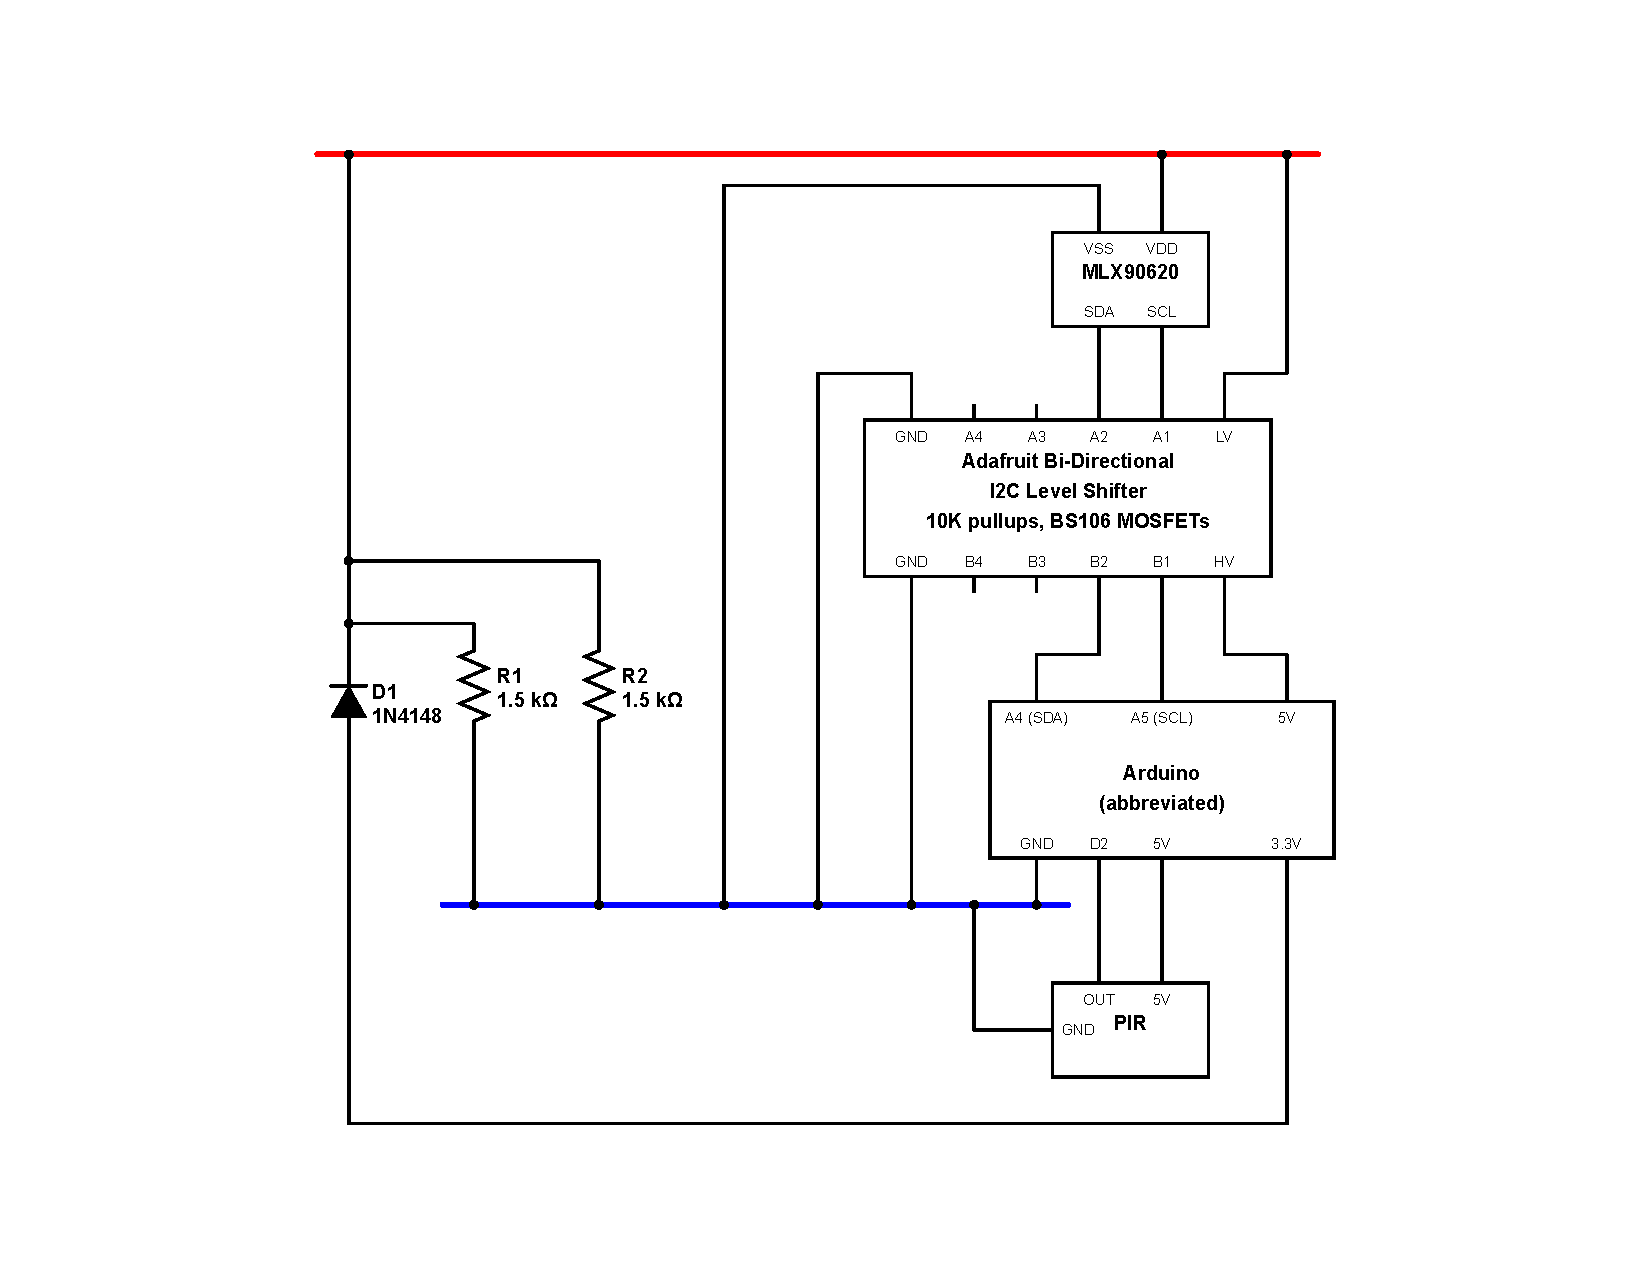
\includegraphics[width=\textwidth]{../diagrams/mlx-arduino.pdf}
\caption{MLX90620, PIR and Arduino integration circuit}
\label{fig:circuits:node}
\end{figure}

Due to low cost and ease of use, the \ard platform was selected as the host for the low-level \iic interface for communication to the \mlx. Initially, this presented some challenges, as the \mlx recommends a power and communication voltage of 2.6V, while the \ard is only able to output 3.3V and 5V as power, and 5V as communication. Due to this, it was not possible to directly connect the \ard to the \mlx, and similarly due to the two-way nature of the \iic 2-wire communication protocol, it was also not possible to simply lower the \ard voltage using simple electrical techniques, as such techniques would interfere with two-way communication.

A solution was found in the form of a \iic level-shifter, the Adafruit ``4-channel I2C-safe Bi-directional Logic Level Converter'' \cite{AdafruitI2C}, which provided a cheap method to bi-directionally communicate between the two devices at their own preferred voltages. The layout of the circuit necessary to link the \ard and the \mlx using this converter can be seen in \Fref{fig:circuits:node}.

Additionally, as used in the Thermosense paper, a \pir motion sensor \cite{AdafruitPIR} was also connected to the \ard. This sensor, operating at 5V natively, did not require any complex circuitry to interface with the \ard. It is connected to digital pin 2 on the \ard, where it provides a rising signal in the event that motion is detected, which can be configured to cause an interrupt on the \ard. In the configuration used in this project, the sensor's sensitivity was set to the highest value (TODO: check) and the timeout for re-triggering was set to the lowest value (approximately 2.5 seconds). Additionally, the continuous re-triggering feature (whereby the sensor produces continuous rising and falling signals for the duration of motion) was disabled using the provided jumpers. 

\subsection{Software}

To calculate the final temperature values that the \mlx offers, a complex initialisation and computational process must be followed, which is specified in the sensor's datasheet \cite{MLXDatasheet}. This process involves initialising the sensor with values attained from a separate on-board \iic EEPROM, then retrieving a variety of normalisation and adjustment values, along with the raw sensor data, to compute the final temperature result.

The basic algorithm to perform this normalisation was based upon code by users ``maxbot'', ``IIBaboomba'', ``nseidle'' and others on the Arduino Forums \cite{ArduinoForum} and was modified to operate with the newer \ard ``Wire'' \iic libraries released since the authors' posts. In pursuit of the project's aims to create a more approachable thermal sensor, the code was also restructured and rewritten to be both more readable, and to introduce a set of features to make the management of the sensor data easier for the user, and for the information to be more human readable.

The first of the features introduced was the human-readable format for serial transmission. This allows the user to both easily write code that can parse the serial to acquire the serial data, as well as examine the serial data directly with ease. When the \ard first boots running the software, the output in \Fref{fig:code:initseq} is output. This specifies several things that are useful to the user; the attached sensor (``DRIVER''), the build of the software (``BUILD'') and the refresh rate of the sensor (``IRHZ''). Several different headers, such as ``ACTIVE'' and ``INIT'' specify the current millisecond time of the processor, thus indicating how long the execution of the initialisation process took (33 milliseconds).

Once booted, the user is able to send several one-character commands to the sensor to configure operation, which are described in \Fref{tab:ardcommands}. Depending on the sensor configuration, IR data may be periodically output automatically, or otherwise manually triggered. This IR data is produced in the packet format described in \Fref{fig:code:packet}. This is a simple, human readable format that includes the millisecond time of the processor at the start and end of the calculation, if the \pir has seen any motion for the duration of the calculation, and the 16x4 grid of calculated temperature values.

\begin{figure}
 \centering
\begin{lstlisting}[style=arduino]
INIT 0
INFO START
DRIVER MLX90620
BUILD Feb  1 2015 00:00:00
IRHZ 1
INFO STOP
ACTIVE 33
\end{lstlisting}
\caption{Initialisation sequence}
\label{fig:code:initseq}
\end{figure}

\begin{table}
\centering
\begin{tabular}{|l|l|}
\hline
\texttt{R} & Flush buffers and reset \ard \\ \hline
\texttt{I} & Print INFO again \\ \hline
\texttt{T} & Activate timers for periodic IR data output \\ \hline
\texttt{O} & Deactivate timers for periodic IR data output \\ \hline
\texttt{P} & Manually trigger capture and output of IR data \\ \hline
\texttt{F\textit{x}} & Set sensor refresh frequency to \textit{x} and reboot \\ \hline
\end{tabular}
\caption{Commands}
\label{tab:ardcommands}
\end{table}

\begin{figure}
 \centering
\begin{lstlisting}[style=arduino]
START 34
MOVEMENT 0
1.0  1.0  1.0  1.0  1.0  1.0  1.0  1.0  1.0  1.0  1.0  1.0  1.0  1.0  1.0  1.0
1.0  1.0  1.0  1.0  1.0  1.0  1.0  1.0  1.0  1.0  1.0  1.0  1.0  1.0  1.0  1.0
1.0  1.0  1.0  1.0  1.0  1.0  1.0  1.0  1.0  1.0  1.0  1.0  1.0  1.0  1.0  1.0
1.0  1.0  1.0  1.0  1.0  1.0  1.0  1.0  1.0  1.0  1.0  1.0  1.0  1.0  1.0  1.0
STOP 97
\end{lstlisting}
\caption{Thermal data packet}
\label{fig:code:packet}
\end{figure}

\begin{figure}
\centering
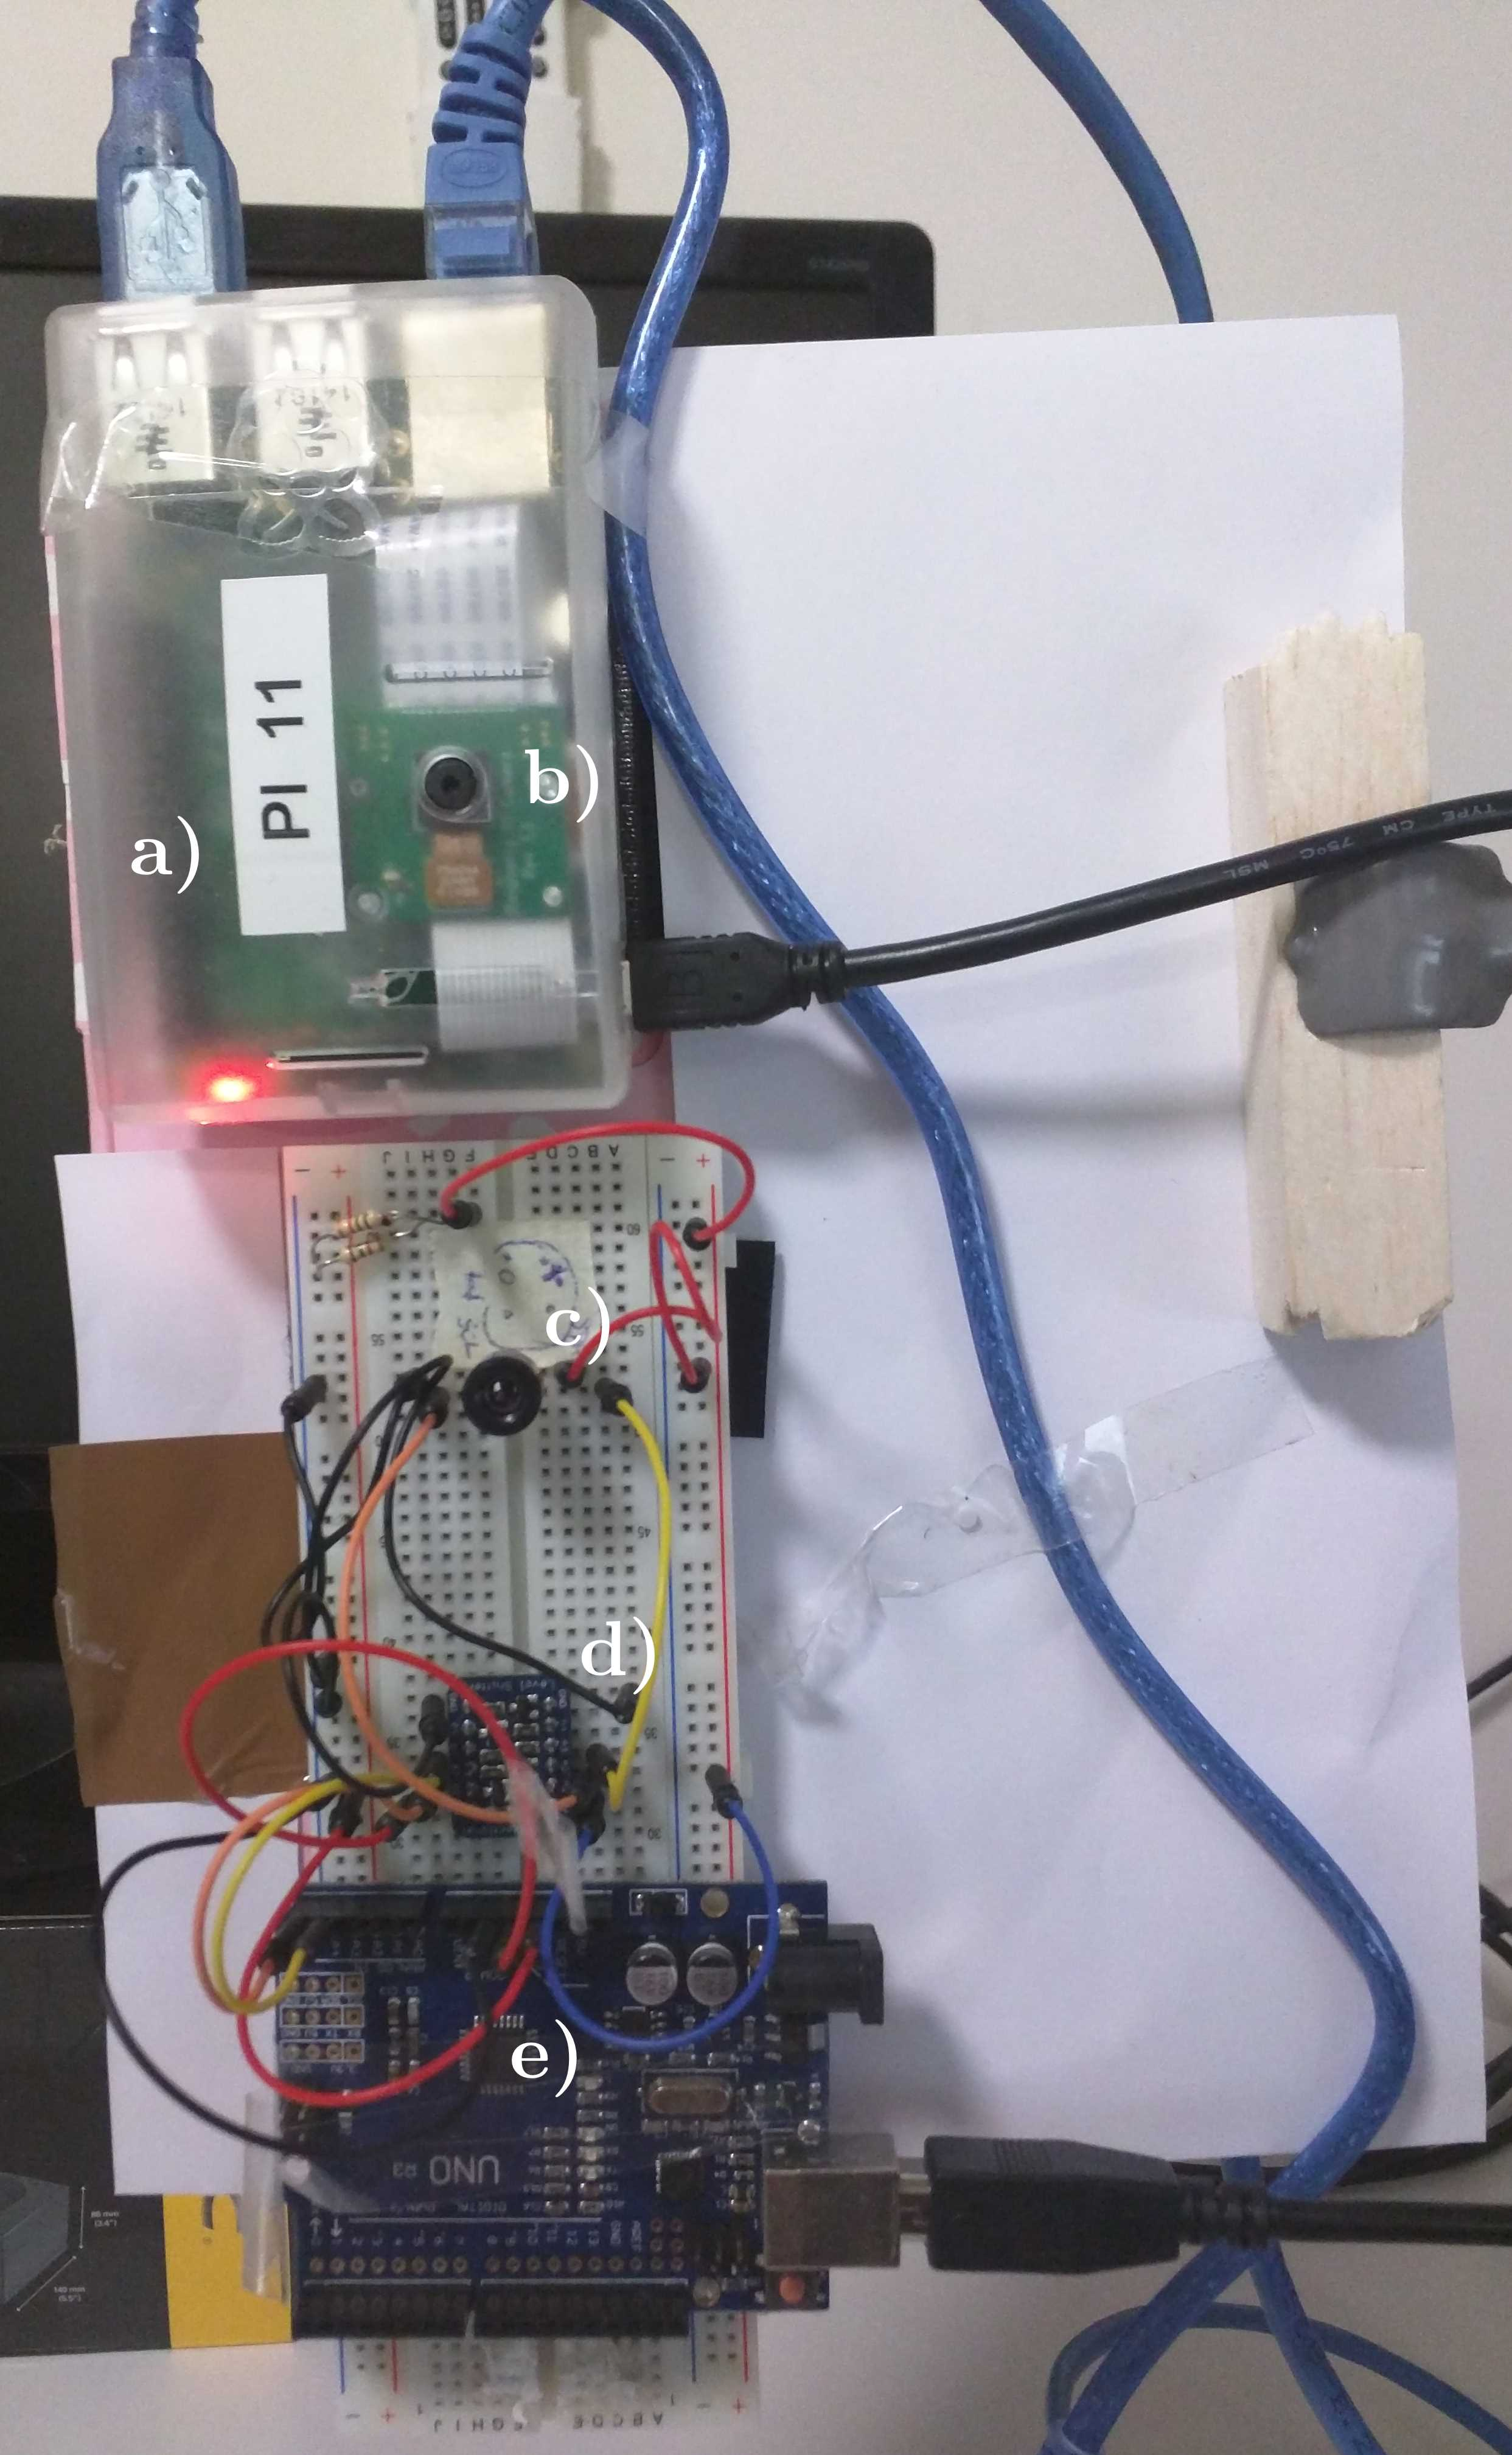
\includegraphics[height=0.7\textheight]{../diagrams/prototypea.jpg}
{\small
\begin{enumerate}[a)]
 \item Raspberry Pi
 \item Camera
 \item \mlx
 \item Level-shifting circuitry
 \item Arduino
\end{enumerate}
}
\caption{Prototype A}
\label{fig:pictures:protoa}
\end{figure}

\begin{figure}
\centering
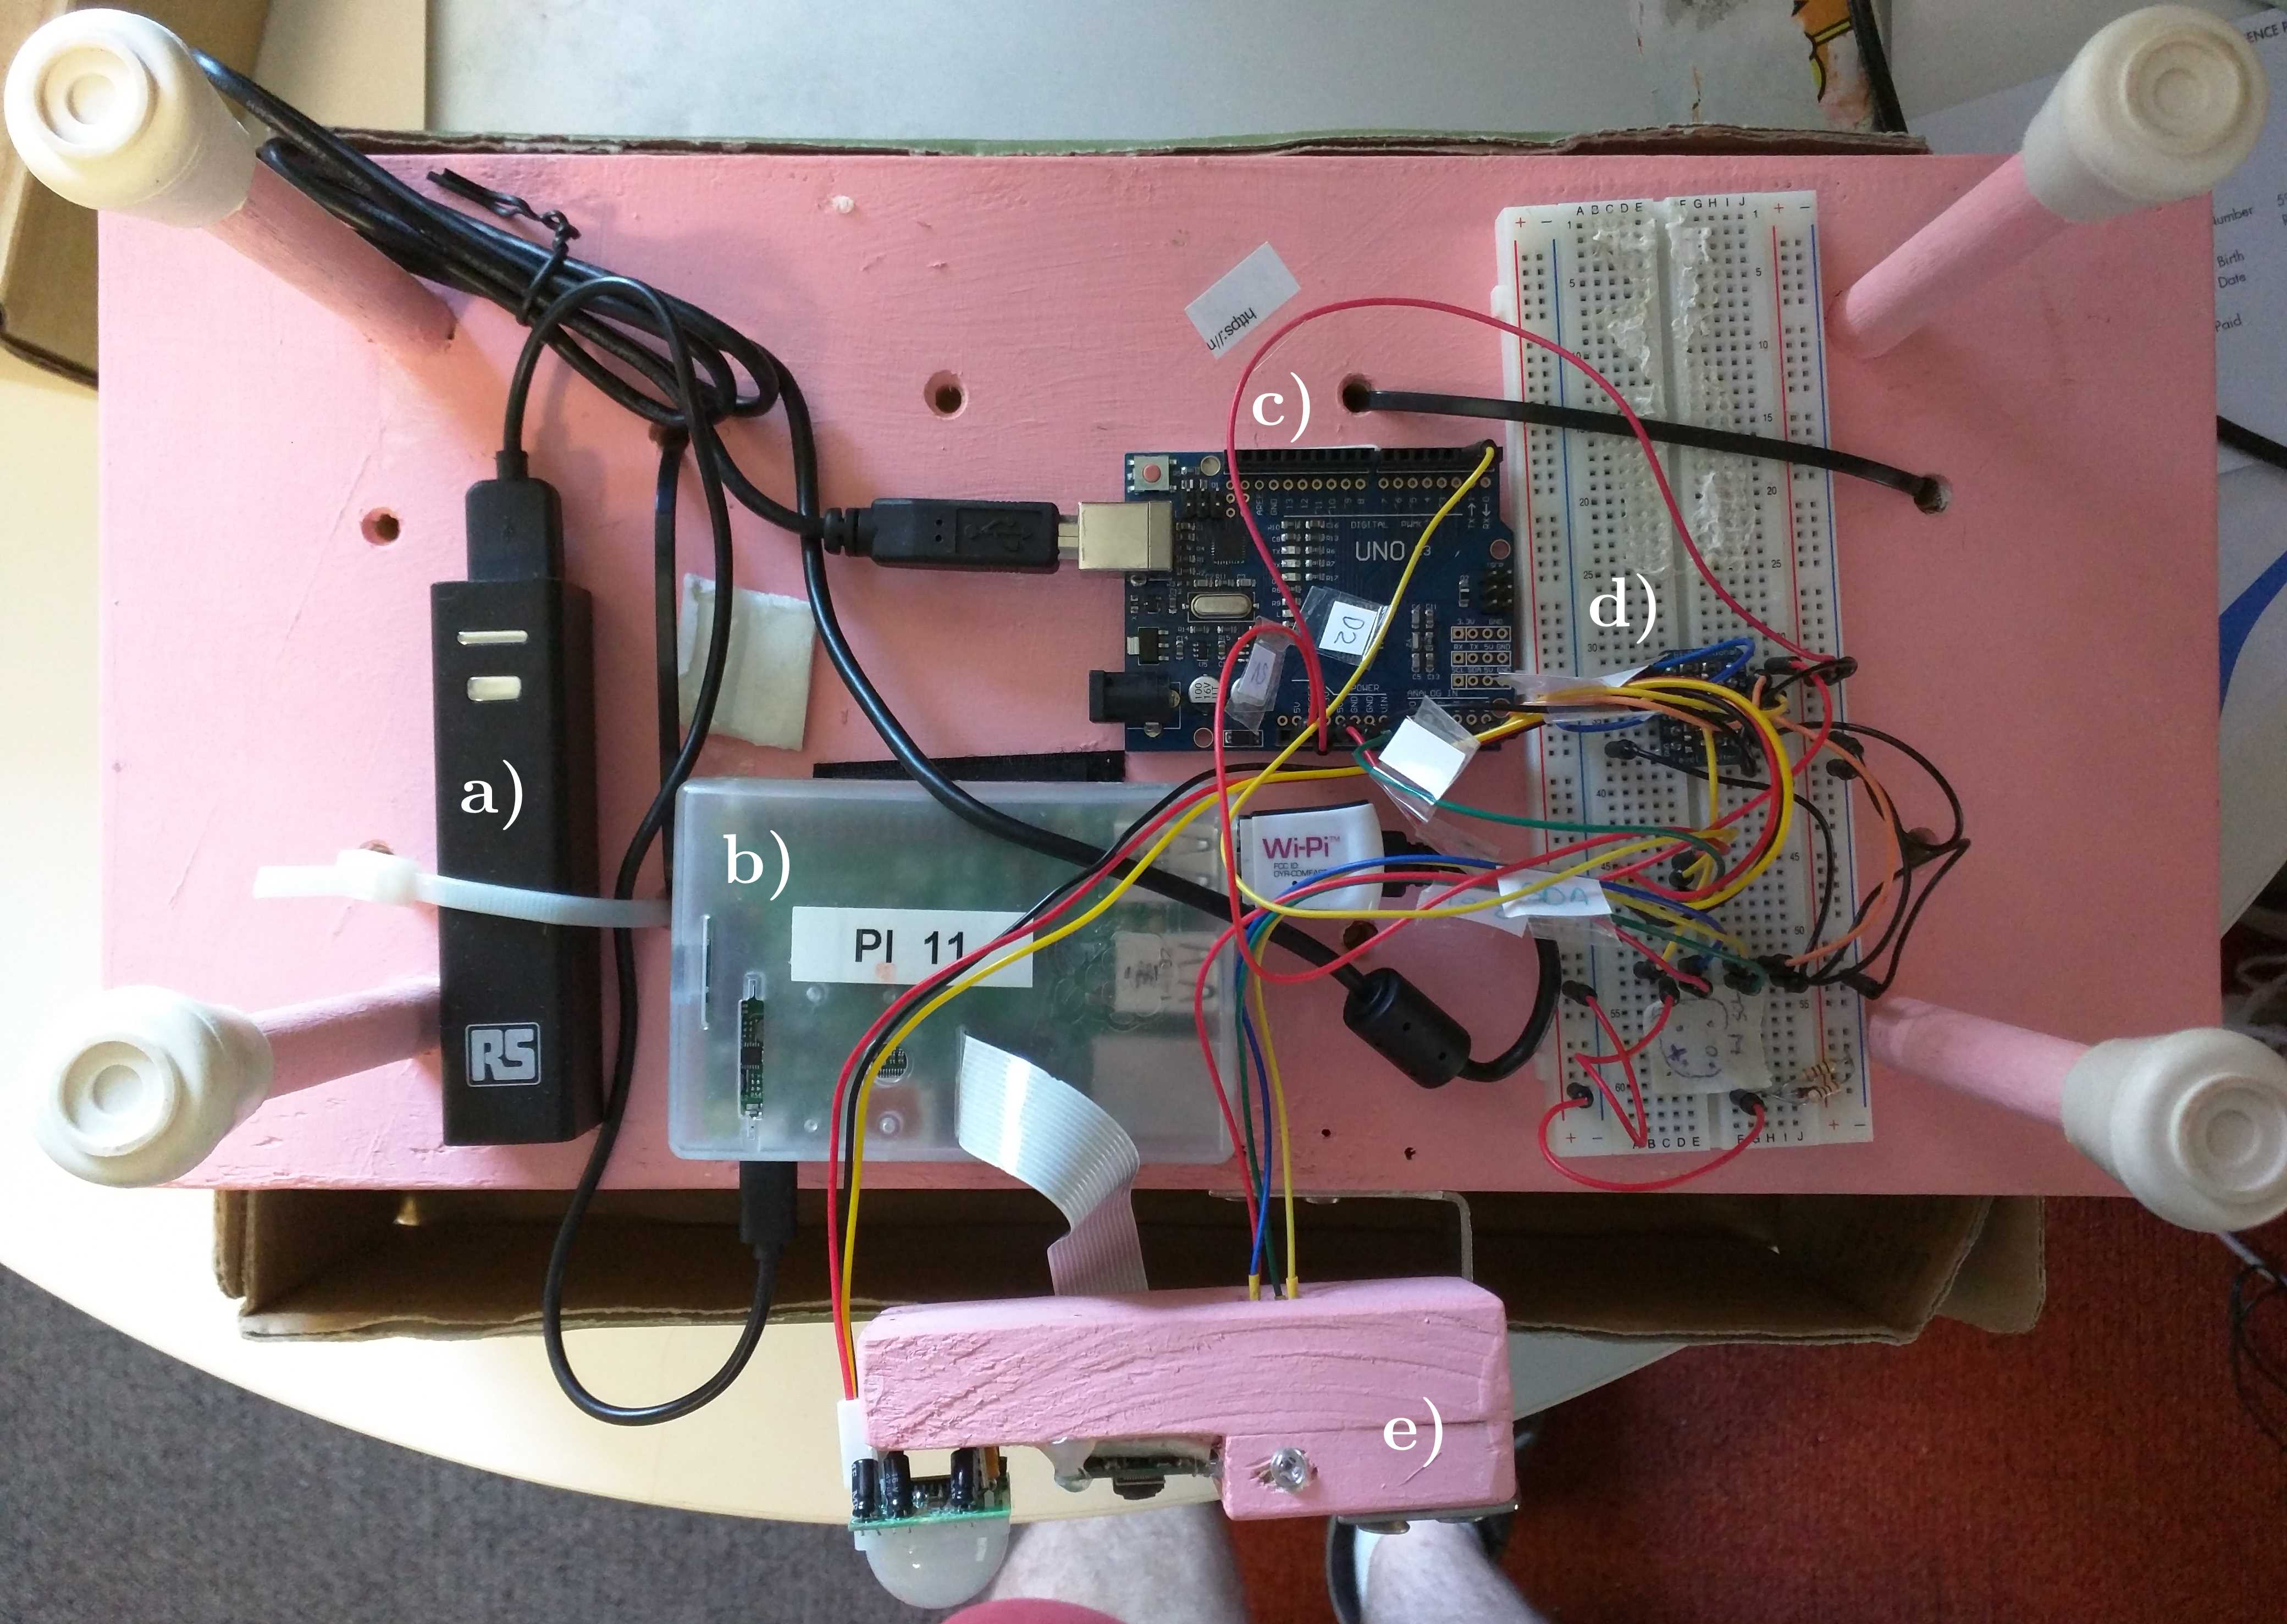
\includegraphics[width=\textwidth]{../diagrams/prototypeb-1.jpg}
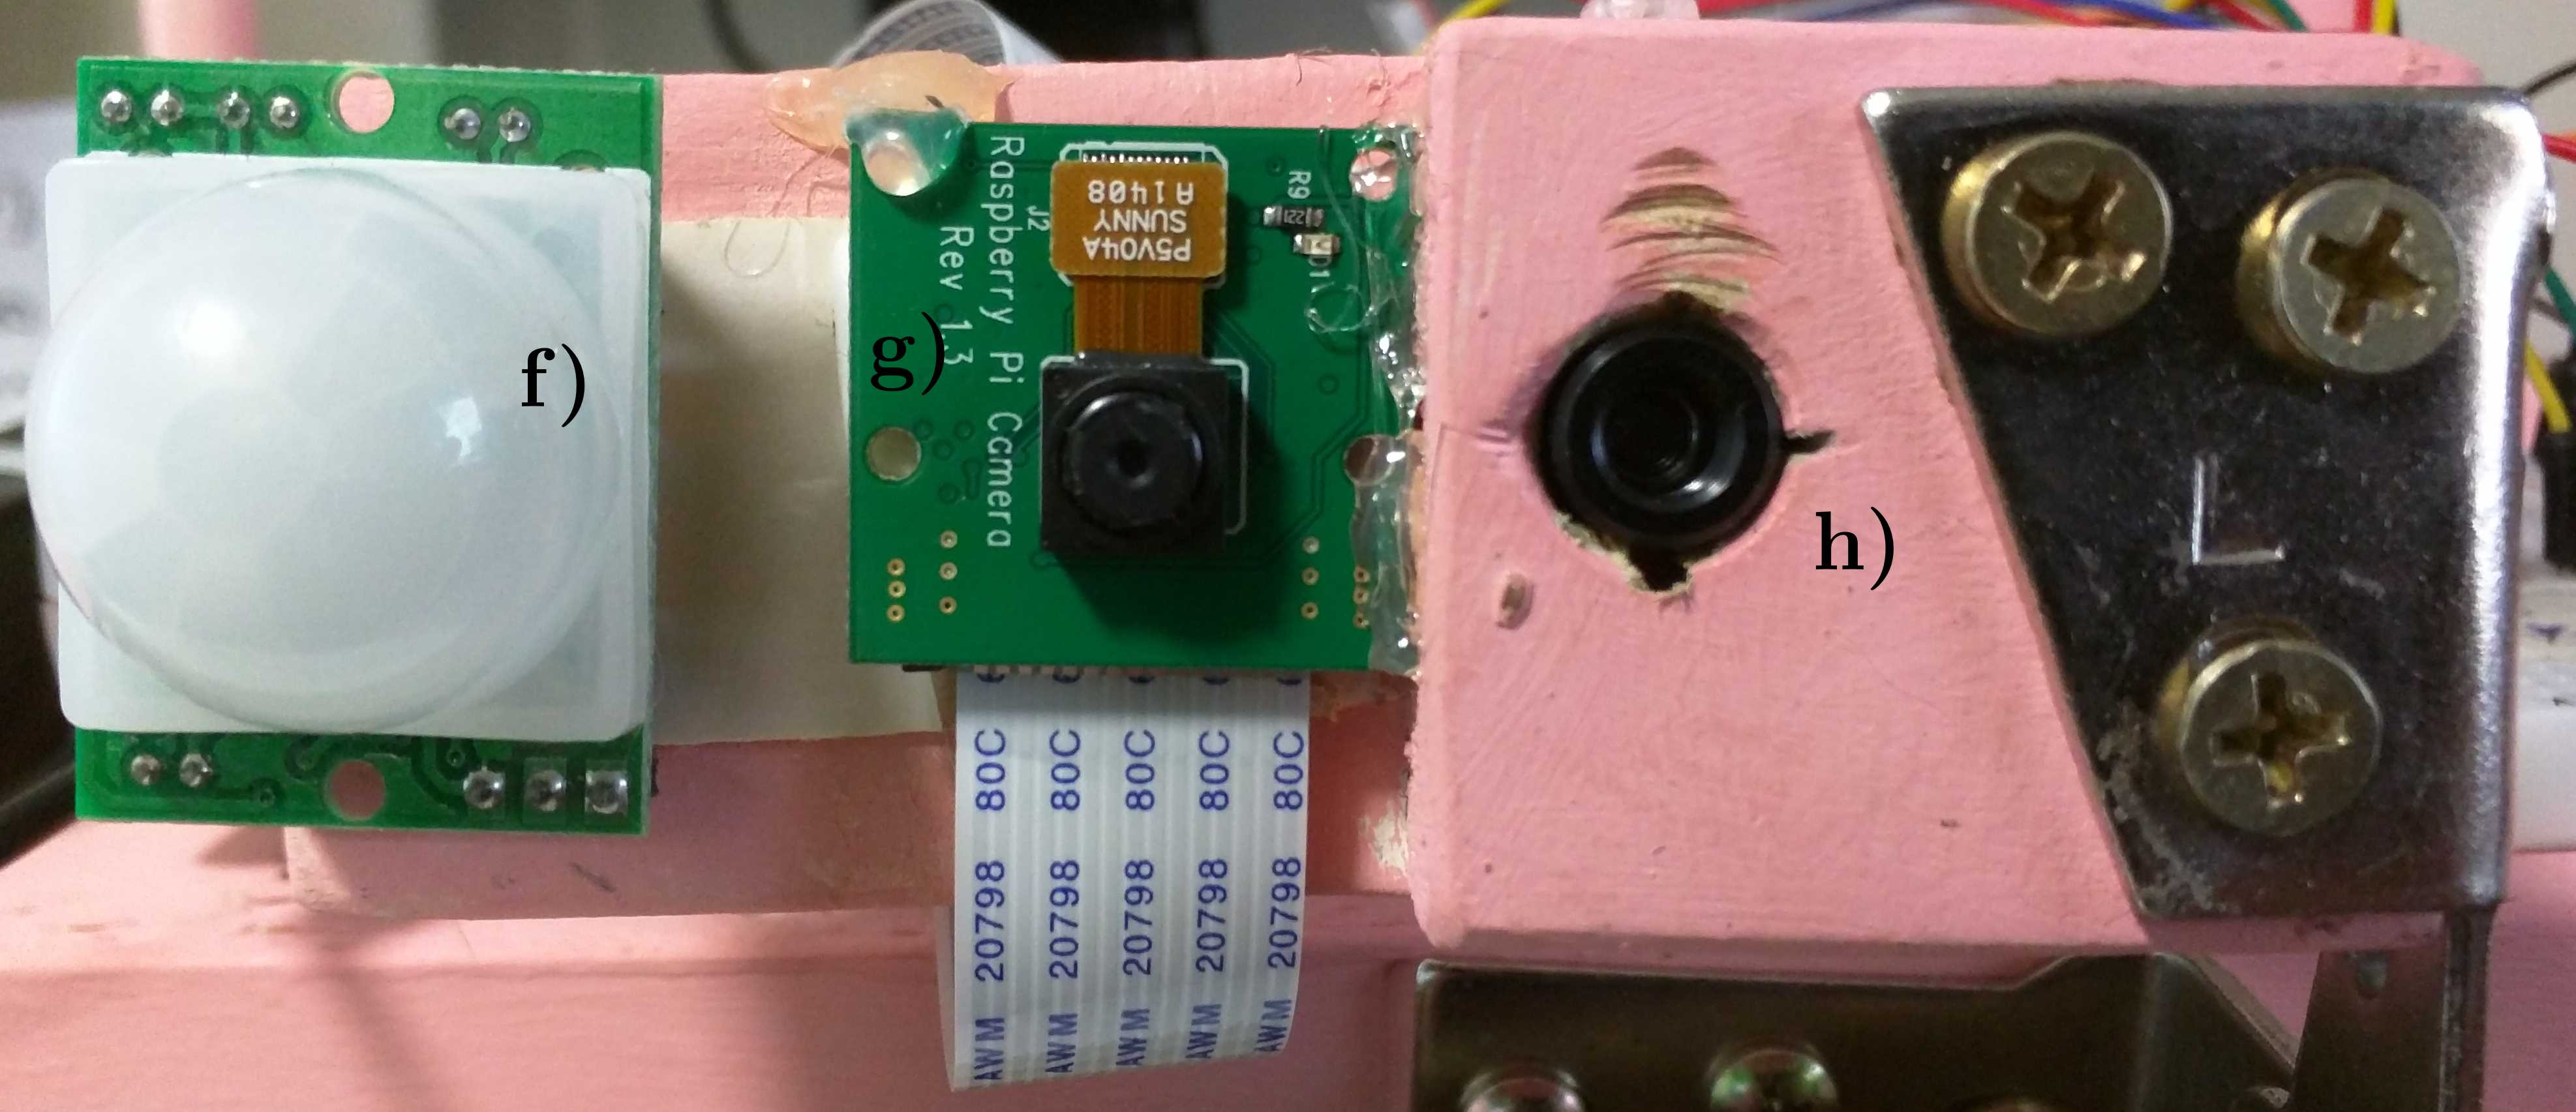
\includegraphics[width=\textwidth]{../diagrams/prototypeb-2.jpg}
{\small
\begin{multicols}{2}
\begin{enumerate}[a)]
 \item Battery pack
 \item Raspberry Pi
 \item Arduino
 \item Level-shifting circuitry
 \item Movable sensor mount
 \item PIR
 \item Camera
 \item \mlx
\end{enumerate}
\end{multicols}
}
\caption{Prototype B}
\label{fig:pictures:protob1}
\end{figure}

\begin{figure}
\centering
\begin{tikzpicture}[node distance=1.7cm]
\node (interwebs) [cbox] {Network};
\node (wifi) [dashbox, right=of interwebs] {\small WiFi / Ethernet};
\node (rpi) [fcont, below=of wifi] {Raspberry Pi \linebreak
  ``Smart Gateway'' \linebreak
  
  \tikz\node[fbox, minimum width=2.3cm, text width=2.3cm] {\small \ttfamily thinglib};
  \tikz\node[fbox, minimum width=2.3cm, text width=2.3cm] {\small \ttfamily features.py};
};
\node (cam) [box, right=of rpi] {Camera};
\node (usb) [dashbox, below=of rpi] {\small USB Serial};
\node (ard) [fcont, below=of usb] {Arduino \linebreak
  ``Sensor'' \linebreak
  
  \tikz\node[fbox, minimum width=3.3cm, text width=3.3cm] {\small \ttfamily mlx90620\_driver};
};
\node (iic) [dashbox, left=of ard] {\small \iic};
\node (mlx) [box, below=of iic] {MLX90620};
\node (wire) [dashbox, right=of ard] {\small Interrupt};
\node (pir) [box, below=of wire] {PIR};

\draw [line] (interwebs) -- (wifi);
\draw [line] (wifi) -- (rpi);
\draw [line] (rpi) -- (usb);
\draw [line] (usb) -- (ard);
\draw [line] (ard) -- (iic);
\draw [line] (iic) -- (mlx);
\draw [line] (ard) -- (wire);
\draw [line] (wire) -- (pir);
\draw [line] (rpi) -- (cam);
\end{tikzpicture}
\caption{Prototype B system architecture}
\label{fig:pictures:protob-arch}
\end{figure}

\ifcsdef{mainfile}{}{\bibliography{../references/primary}}
\end{document}